\section*{Problem 1}
\subsection*{Part a}
\eq{
E_{stark} &= -\frac{\hbar}{4\delta}|\Omega|^2\\
&= -\frac{d^2}{4\hbar\delta}|E|^2\\
&= -\frac{d^2}{4\hbar\delta}E_0^2e^{-\frac{2}{\omega_0^2}(x^2+y^2)}
}
Assuming the atom is at $x=y=0$
\eq{
E_{stark} &= -\frac{d^2E_0^2}{4\hbar\delta}
}
\subsection*{Part b}
Approximating the Stark energy shift to second order
\eq{
E_{stark} &= -\frac{d^2E_0^2}{4\hbar\delta}\sum_k(-\frac{2}{\omega_0^2})^k\frac{1}{k!}(x^2+y^2)^k\\
&=-\frac{d^2E_0^2}{4\hbar\delta}\sum_{k=0}^\infty(-\frac{2}{\omega_0^2})^k\frac{1}{k!}\sum_{j=0}^k\binom{k}{j}x^{2j}y^{2(k-j)}\\
&= -\frac{d^2E_0^2}{4\hbar\delta} (1-\frac{2}{\omega_0^2}(x^2+y^2))
}
If we take the potential to be the shifted energy then
\eq{
V &= -\frac{d^2E_0^2}{4\hbar\delta} (1-\frac{2}{\omega_0^2}(x^2+y^2))\\
V_{qho} &= \frac{1}{2}m_e\omega^2(x^2+y^2)
}
If we disregard the constant offset we can identify the oscillator frequency
\eq{
\omega^2 &= \frac{d^2E_0^2}{m_e\hbar\delta\omega_0^2}\\
\omega &= (\frac{d^2 E_0^2}{m_e \hbar \delta \omega_0^2})^{ 1/2 }
}
\subsection*{Part c}
First we have to calculate the magnitude of the electric field in terms of the power
\eq{
P_{AVG} &= \int \Vec{S}_{AVG}\cdot d\Vec{A}\\
&= \int \frac{r}{2\mu_0} (\Vec{E}\times\Vec{B}) \cdot d\Vec{A}\\
&= \int \frac{1}{2c\mu_0} E_0^2 e^{-\frac{2}{\omega_0^2}(r^2)}drd\theta\\
&= \frac{\pi}{\mu_0 c}E_0^2 \int_0^\infty r e^{-\frac{2}{\omega_0^2}(r^2)}dr\\
&= \pi\epsilon_0 c E_0^2 \frac{\omega_0^2}{4}
}
Plugging this into the answer for part b we get
\eq{
\omega &= (\frac{e^2a_0^2}{m_e\hbar\delta\omega_0^2}\frac{4P}{\pi c \epsilon_0 \omega_0^2})^{ 1/2 }\\
&\approx 18.945 MHz
}
The code for calculating the value is in the appendix.
\subsection*{Part d}
In temperature units
\eq{
\omega \times \frac{\hbar}{k_B} &= 18.945 MHz \times \frac{1.054571817e-34 Js}{1.380649e-23 J/K }\\
&\approx 0.145 mK
}
\newpage
\section*{Problem 2}
\subsection*{Part a}
The first order correction to the Fock state $\ket{\psi_m}$ is
\eq{
\ket{\psi_n^{(1)}} &= \sum_{m} \frac{\braket{\psi_m^{(0)}|H'|\psi_n^{(0)}}}{E_n-E_m}\ket{\psi_m^{(0)}}
}
Where $m=0,\dots,n-1,n+1,\dots$.
The $n$'th energy level of the harmonic oscillator is
\eq{
E_n &= (n+ 1/2 )\hbar \omega\\
\implies E_n-E_m &= (n-m)\hbar \omega
}
When $H' = x^k$
\eq{
\braket{\psi_m^{(0)}|H'|\psi_n^{(0)}} &= \braket{\psi_m^{(0)}|x^k|\psi_n^{(0)}}\\
&= (\frac{\hbar}{2m\omega})^{ k/2 }\braket{\psi_m^{(0)}|(\hat{a}^\dag + \hat{a})^k|\psi_n^{(0)}}
}
Clearly, this product must go to $0$ if $m < n - k$ or $m > n + k$. Similarly, unless $n+k \equiv_2 m$ this product goes to $0$.\\


When $k=4$ the only valid $m$ states are $2,4$ and $3,5$, for ground and first excited state, respectively. These are simple enough combinations to do by hand.
\eq{
\ket{\psi_0^{(1)}} &= -\frac{\lambda}{\hbar \omega}\sum_{m} \frac{\braket{\psi_m^{(0)}|x^4|\psi_0^{(0)}}}{m}\ket{\psi_m^{(0)}}\\
&= -\frac{\lambda}{\hbar\omega}(\frac{1}{2}\braket{\psi_2|x^4|\psi_0}\ket{\psi_2}+\frac{1}{4}\braket{\psi_4|x^4|\psi_0}\ket{\psi_4})\\
&= -\frac{\lambda\hbar}{4m^2\omega^3}(3\sqrt{2}\ket{\psi_2}+ \frac{\sqrt{6}}{2}\ket{\psi_4})\\
}
\eq{
\ket{\psi_1^{(1)}} &= \frac{\lambda}{\hbar\omega}\sum_{m} \frac{\braket{\psi_m^{(0)}|x^4|\psi_1^{(0)}}}{1-m}\ket{\psi_m^{(0)}}\\
&= -\frac{\lambda}{\hbar\omega}(\frac{1}{2}\braket{\psi_3|x^4|\psi_1}\ket{\psi_3}+\frac{1}{4}\braket{\psi_5|x^4|\psi_1}\ket{\psi_5})\\
&= -\frac{\lambda\hbar}{4m^2\omega^3}(\frac{\sqrt{3}(\sqrt{2}+2\sqrt{6})}{2}\ket{\psi_3}+\frac{\sqrt{30}}{4}\ket{\psi_5})
}

\subsection*{Part b}
The second order correction to energy goes as
\eq{
E_n^{(2)} = \sum \frac{|\braket{\psi_m^{(0)}|\lambda x^k|\psi_n^{(0)}}|^2}{E_n-E_m}
}
Where again we only need to sum over $m=2,4$ and $m=3,5$
\eq{
E_0^(2) &= -\frac{\lambda^2}{\hbar \omega}\sum_{m} \frac{|\braket{\psi_m^{(0)}|x^4|\psi_0^{(0)}}|^2}{m}\\
&= -\frac{\lambda^2}{\hbar\omega}(\frac{1}{2}|\braket{\psi_2|x^4|\psi_0}|^2+\frac{1}{4}|\braket{\psi_4|x^4|\psi_0}|^2)\\
&= -\frac{\lambda^2\hbar}{4m^2\omega^3}(6^2+ 12)\\
}
\eq{
E_1^(2) &= -\frac{\lambda^2}{\hbar \omega}\sum_{1-m} \frac{|\braket{\psi_m^{(0)}|x^4|\psi_1^{(0)}}|^2}{m}\\
&= -\frac{\lambda^2}{\hbar\omega}(\frac{1}{2}|\braket{\psi_3|x^4|\psi_0}|^2+\frac{1}{4}|\braket{\psi_5|x^4|\psi_0}|^2)\\
&= -\frac{\lambda^2\hbar}{4m^2\omega^3}(3(\sqrt{2}+2\sqrt{6})^2+30)\\
}

\subsection*{Part c}
The first two eigen-energies are $E_0 = 0.507$ and $E_1 = 1.535$ via QuTip -see code appendix.\\

To compare we first have to calculate the first order correction to the eigen-energies
\eq{
E_0^(1) &= \braket{\psi_0^{(0)}|H'|\psi_0^(0)}\\
&= \lambda \braket{\psi_0^{(0)}|x^4|\psi_0^(0)}\\
&= \lambda (\frac{\hbar}{2m\omega})^2\braket{\psi_0^{(0)}|(\hat{a}+\hat{a}^\dag)^4|\psi_0^(0)}\\
&= \lambda (\frac{\hbar}{2m\omega})^23
}
\eq{
E_1^(1) &= \lambda (\frac{\hbar}{2m\omega})^2\braket{\psi_1^{(0)}|(\hat{a}+\hat{a}^\dag)^4|\psi_1^(0)}\\
&= \lambda (\frac{\hbar}{2m\omega})^215
}
Plugging in values to part a and b, we can calculate the second order correction to energy for the ground and first excited state
\eq{
\frac{E_0}{\hbar} &\approx 0.5 + (0.01)\hbar \cdot 0.75 - (0.01)^2\cdot 12\\
&\approx 0.499\\
\frac{E_1}{\hbar} &\approx 1.5 + (0.01)\hbar \cdot 3.75 - (0.01)^2\cdot 37.39 \\
&\approx 1.497
}
This is roughly what we expect, a bit lower, if we keep going in the expansion it will eventually converge.
\newpage
\section*{Problem 3}
\subsection*{Part a}
\eq{
\ket{\psi_1} &= \frac{1}{\sqrt{2}}(\ket{\uparrow}+\ket{\downarrow})\\
\ket{\psi_2} &= \ket{\uparrow}
}
The total state vector is
\eq{
\ket{\psi} &= \frac{1}{\sqrt{2}}(\ket{\uparrow\uparrow}+\bra{\downarrow\uparrow})
}
The expectation value of $\braket{\sigma_z^{(1)}}$ is
\eq{
\braket{\sigma_z\otimes \sigma_0} &= \frac{1}{2}(\bra{\uparrow\uparrow}+\bra{\downarrow\uparrow})\sigma_z\otimes \sigma_0(\ket{\uparrow\uparrow}+\bra{\downarrow\uparrow})\\
&= 1/2 \braket{\uparrow\uparrow| \sigma_z\otimes \sigma_0 | \uparrow\uparrow} + 1/2 \braket{\uparrow\uparrow| \sigma_z\otimes \sigma_0 | \downarrow\uparrow}\\
&+ 1/2 \braket{\downarrow\uparrow| \sigma_z\otimes \sigma_0 | \uparrow\uparrow} + 1/2 \braket{\downarrow\uparrow| \sigma_z\otimes \sigma_0| \downarrow\uparrow}\\
&= 1/2 ( 1 \cdot 1 - 1 \cdot 1 + 1\cdot 1 - 1 \cdot 1)\\
&= 0
}
The expectation value of $\braket{\sigma_z^{(2)}}$ is
\eq{
\braket{\sigma_0 \otimes \sigma_z} &= \frac{1}{2}(\bra{\uparrow\uparrow}+\bra{\downarrow\uparrow})\sigma_0 \otimes \sigma_z(\ket{\uparrow\uparrow}+\bra{\downarrow\uparrow})\\
&= 1/2 \braket{\uparrow\uparrow| \sigma_0 \otimes \sigma_z | \uparrow\uparrow} + 1/2 \braket{\uparrow\uparrow| \sigma_0 \otimes \sigma_z | \downarrow\uparrow}\\
&+ 1/2 \braket{\downarrow\uparrow| \sigma_0 \otimes \sigma_z | \uparrow\uparrow} + 1/2 \braket{\downarrow\uparrow| \sigma_0 \otimes \sigma_z| \downarrow\uparrow}\\
&= 1/2 ( 1 \cdot 1 + 0 \cdot 1 + 0\cdot 1 + 1 \cdot 1)\\
&= 1
}
The expectation value of $\braket{\sigma_z^{(1)}\otimes \sigma_z^{(2)}}$ is
\eq{
\braket{\sigma_z\otimes \sigma_z} &= \frac{1}{2}(\bra{\uparrow\uparrow}+\bra{\downarrow\uparrow})\sigma_z \otimes \sigma_z(\ket{\uparrow\uparrow}+\bra{\downarrow\uparrow})\\
&= 1/2 \braket{\uparrow\uparrow| \sigma_z \otimes \sigma_z | \uparrow\uparrow} + 1/2 \braket{\uparrow\uparrow| \sigma_z \otimes \sigma_z | \downarrow\uparrow}\\
&+ 1/2 \braket{\downarrow\uparrow| \sigma_z \otimes \sigma_z | \uparrow\uparrow} + 1/2 \braket{\downarrow\uparrow| \sigma_z \otimes \sigma_z| \downarrow\uparrow}\\
&= 1/2 ( 1 \cdot 1 - 0 \cdot 1 + 0\cdot 1 - 1 \cdot 1)\\
&= 0
}

\subsection*{Part b}
\eq{
\ket{\psi_1} &= \frac{1}{\sqrt{2}}(\ket{\uparrow}+\ket{\downarrow})\\
\ket{\psi_2} &= \frac{1}{\sqrt{2}}(\ket{\uparrow}+\ket{\downarrow})
}
So the total state vector is
\eq{
\ket{\psi} &= 1/2 (\ket{\uparrow\uparrow}+\ket{\uparrow\downarrow}+\ket{\downarrow\uparrow}+\ket{\downarrow\downarrow})
}
The expectation value of $\braket{\sigma_z^{(1)}\otimes \sigma_z^{(2)}}$ is
\eq{
\braket{\sigma_z^{(1)}\otimes \sigma_z^{(2)}} &= \braket{\psi|\sigma_z\otimes \sigma_z|\psi}\\
&= 1/4 \braket{\uparrow\uparrow|\sigma_z\otimes \sigma_z|\uparrow\uparrow}+ 1/4 \braket{\uparrow\downarrow|\sigma_z\otimes \sigma_z|\uparrow\downarrow}\\
&+ 1/4 \braket{\downarrow\uparrow|\sigma_z\otimes \sigma_z|\downarrow\uparrow}+ 1/4 \braket{\downarrow\downarrow|\sigma_z\otimes \sigma_z|\downarrow\downarrow}\\
&= 1/4 (1\cdot1 - 1\cdot 1 - 1\cdot 1 + 1\cdot 1)\\
&= 0
}
Where I prematurely dropped terms that would just go to $0$. The expectation value of $\braket{\sigma_x^{(1)}\otimes \sigma_x^{(2)}}$ is
\eq{
\braket{\sigma_x^{(1)}\otimes \sigma_x^{(2)}} &= \braket{\psi|\sigma_x\otimes \sigma_x|\psi}\\
&= 1/4 \braket{\uparrow\uparrow|\sigma_x\otimes \sigma_x|\downarrow\downarrow}+ 1/4 \braket{\downarrow\downarrow|\sigma_x\otimes \sigma_x|\uparrow\uparrow}\\
&+ 1/4 \braket{\downarrow\uparrow|\sigma_x\otimes \sigma_x|\uparrow\downarrow}+ 1/4 \braket{\uparrow\downarrow|\sigma_x\otimes \sigma_x|\downarrow\uparrow}\\
&= 1/4 (1\cdot1 + 1\cdot 1 + 1\cdot 1 + 1\cdot 1)\\
&= 1
}

\subsection*{Part c}
The total state vector
\eq{
\ket{\psi} &= \frac{1}{\sqrt{2}} (\ket{\uparrow\uparrow}+\ket{\downarrow\downarrow})\\
}
The expectation value of $\braket{\sigma_z^{(1)}\otimes \sigma_z^{(2)}}$
\eq{
\braket{\sigma_z^{(1)}\otimes \sigma_z^{(2)}} &= 1/2 (\bra{\uparrow\uparrow}+\bra{\downarrow\downarrow})\sigma_z\otimes \sigma_z(\ket{\uparrow\uparrow})+\ket{\downarrow\downarrow})\\
&= 1/2 (\bra{\uparrow \uparrow}\sigma_z\otimes \sigma_z\ket{\uparrow\uparrow}+\bra{\downarrow \downarrow}\sigma_z\otimes \sigma_z\ket{\downarrow\downarrow})\\
&= 1/2 (1+1)\\
&= 1
}

The expectation value of $\braket{\sigma_x^{(1)}\otimes \sigma_x^{(2)}}$
\eq{
\braket{\sigma_x^{(1)}\otimes \sigma_x^{(2)}} &= 1/2 (\bra{\uparrow\uparrow}+\bra{\downarrow\downarrow})\sigma_x\otimes \sigma_x(\ket{\uparrow\uparrow})+\ket{\downarrow\downarrow})\\
&= 1/2 (\bra{\uparrow \uparrow}\sigma_x\otimes \sigma_x\ket{\downarrow\downarrow}+\bra{\downarrow \downarrow}\sigma_x\otimes \sigma_x\ket{\uparrow\uparrow})\\
&= 1/2 (1+1)\\
&= 1
}

\subsection*{Part d}
\eq{
\ket{\psi_1} &= a_1 \ket{\uparrow} + b_1 \ket{\downarrow}\\
\ket{\psi_2} &= a_2 \ket{\uparrow} + b_2 \ket{\downarrow}\\
\ket{\psi_3} &= a_3 \ket{\uparrow} + b_3 \ket{\downarrow}\\
}
The total state vector is
\eq{
\ket{\psi} &= \ket{\psi_1}\otimes\ket{\psi_2}\otimes\ket{\psi_3}\\
&=(a_1a_2\ket{\uparrow\uparrow}+a_1b_2\ket{\uparrow\downarrow}+b_1a_2\ket{\downarrow\uparrow}+b_1b_2\ket{\downarrow\downarrow})\otimes\ket{\psi_3}\\
&=a_1a_2a_3\ket{\uparrow\uparrow\uparrow}+a_1b_2a_3\ket{\uparrow\downarrow\uparrow}+b_1a_2a_3\ket{\downarrow\uparrow\uparrow}+b_1b_2a_3\ket{\downarrow\downarrow\uparrow}\\
&+a_1a_2b_3\ket{\uparrow\uparrow\downarrow}+a_1b_2b_3\ket{\uparrow\downarrow\downarrow}+b_1a_2b_3\ket{\downarrow\uparrow\downarrow}+b_1b_2b_3\ket{\downarrow\downarrow\downarrow}
}

\subsection*{Part e}
\eq{
\ket{\psi} &= a_1 \ket{\uparrow}+b_1\ket{\downarrow}\\
\ket{\phi} &= \frac{1}{\sqrt{3}}(\ket{\psi_0}+\ket{\psi_1}+\ket{\psi_3})
}
The total state vector is
\eq{
\ket{\xi} &= \ket{\psi}\otimes\ket{\phi}\\
&= \frac{a_1}{\sqrt{3}}(\ket{\uparrow \psi_0}+\ket{\uparrow \psi_1}+\ket{\uparrow \psi_3})\\
&+ \frac{b_1}{\sqrt{3}}(\ket{\downarrow \psi_0}+\ket{\downarrow \psi_1} + \ket{\downarrow \psi_3})
}
The expectation value of $\braket{\sigma_z}$ is
\eq{
\braket{\sigma_z} &= \braket{\xi | \sigma_z \otimes I | \xi}\\
&= \frac{a_1^2}{3}(\braket{\uparrow \psi_0 | \uparrow \psi_0} + \braket{\uparrow \psi_1|\uparrow \psi_1}+\braket{\uparrow \psi_3|\uparrow \psi_3})\\
&- \frac{b_1^2}{3}(\braket{\downarrow \psi_0|\downarrow \psi_0}+\ket{\downarrow \psi_1|\downarrow \psi_1}+\ket{\downarrow \psi_3 | \downarrow \psi_3})\\
&= a_1^2 - b_1^2
}
The expectation value of $\hat{N}$ is
\eq{
\braket{\hat{N}} &= \braket{\xi | \sigma_0 \otimes \hat{N} | \xi}\\
&= \frac{a_1^2}{3}(0\cdot\braket{\uparrow \psi_0 | \uparrow \psi_0} + 1\cdot\braket{\uparrow \psi_1|\uparrow \psi_1}+3\cdot\braket{\uparrow \psi_3|\uparrow \psi_3})\\
&+ \frac{b_1^2}{3}(0\cdot\braket{\downarrow \psi_0|\downarrow \psi_0}+1\cdot\ket{\downarrow \psi_1|\downarrow \psi_1}+3\cdot\ket{\downarrow \psi_3 | \downarrow \psi_3})\\
&= 4/3 (a_1^2 + b_1^2)\\
&= 4/3
}
The probability of finding our system in state $\ket{\downarrow \psi_3}$ is
\eq{
P_{\ket{\downarrow \psi_3}} &= \frac{|b_1|^2}{3}
}
\newpage
\section*{Problem 4}
\subsection*{Part a}
The Hamiltonian and time evolution operator were defined in QuTip and I used Matplotlib to plot the resulting graphs. The Python code is in the appendix.
\begin{figure}[h]
    \centering
    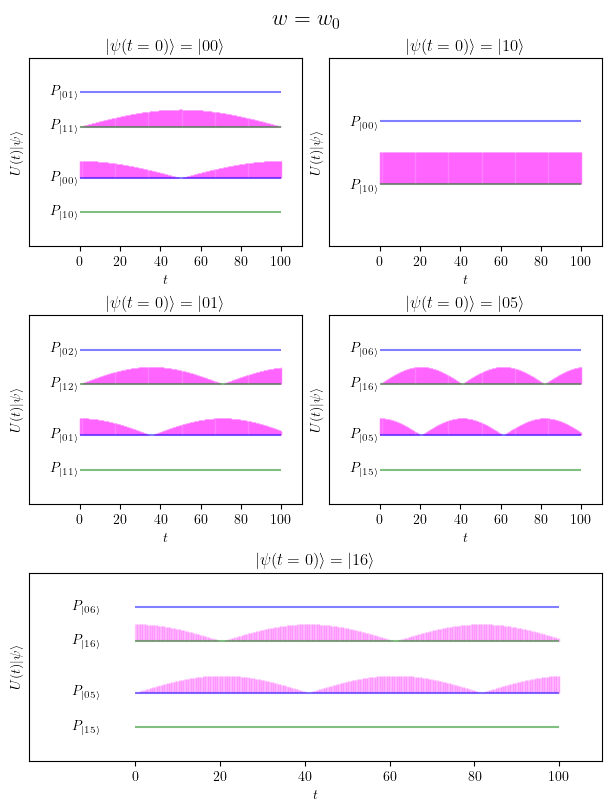
\includegraphics[width=0.85\linewidth]{Resources//245//Homework 6/245 Homework 6 Problem 4a.png}
\end{figure}
\pagebreak
\subsection*{Part b}
I plotted the probability distribution of being in each state on the Jaynes-Cummings ladder.
\begin{figure}[h]
    \centering
    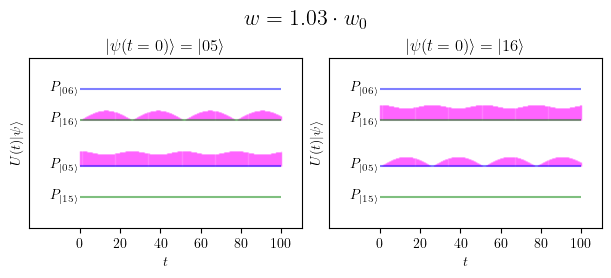
\includegraphics[width=1\linewidth]{Resources//245//Homework 6/245 Homework 6 Problem 4b.png}
\end{figure}
\newpage
\section*{Code Appendix}
\subsection*{Problem 1}
\begin{python}
from numpy import sqrt, pi

e = 1.60217646*10**-19 #C
a0 = 5.29177210903*10**-11 #m
w0 = 10*10**-6 #m
me = 9.10938188*10**-31 #kg
hbar = 1.054571817*10**-34 #Js
delta = 10*10**12 #Hz
c = 299792458 #m/s
epsilon0 = 8.8541878188*10**-12 #(C^2s^2)/(m^3kg)
P = 100*10**-3 #W
kB = 1.380649*10**-23 #J/K

w = sqrt((e**2*a0**2*4*P)/(me*hbar*delta*pi*c*epsilon0*w0**4))

w*(hbar/kB)*10**3

\end{python}
\subsection*{Problem 2}
\begin{python}
from qutip import position, momentum

w = 1
lam = 0.01
m = 1
nmax = 10

K = (momentum(nmax)**2)/(2*m) + (m*w**2/2)*position(nmax)**2
V = lam*position(nmax)**4
H = K + V

E = H.eigenenergies()
\end{python}
\subsection*{Problem 4}

\begin{python}
# Problem 4
from qutip import states, tensor, expect, ket
from qutip import sigmaz as sz
from qutip import sigmax as sx
from qutip import sigmap as sp
from qutip import sigmam as sm
from qutip import qeye as I
from qutip import create, destroy

from numpy import sqrt, pi, linspace, absolute, sum
from numpy import ndarray

import matplotlib.pyplot as plt

flatten = ndarray.flatten
fock = states.fock
base = states.basis

def H(w0, w, g, N):
    Hqubit = tensor((w0/2)*sz(),I(N))
    Hqho = w*(tensor(I(2), create(N)*destroy(N))+0.5)
    Hint = (g/2)*(tensor(sp(), destroy(N))+tensor(sm(), create(N)))

    return Hqubit + Hqho + Hint

def U(t, w0, w, g, N):
    return (-1j*H(w0, w, g, N)*t).expm()

def Psi(spin, n, N):
    return tensor(fock(2,spin),base(N,n))

def JCumLadPlot(tpoints, psi, N, title, ax):
    plt.rcParams.update({
        "text.usetex": True,
        "font.family": "Serif"
    })

    dims = linspace(0,N-1,N,dtype=int)
    maxt = max(tpoints)

    # Extract probabilities from list of states psi
    psi_coeff = [[absolute(p[0:N]),absolute(p[N:2*N])] for p in psi]
    
    # Determine non-zero dimensions to plot
    qho_list = dims[flatten(sum([sum(psi_coeff[i],axis=0) for i in linspace(0,len(tpoints)-1,len(tpoints),dtype=int)],axis=0) != 0.0)]
    
    # Spacing parameters for horizontal lines
    a = 1
    b = 1.5
    nqhostates = len(qho_list)

    # Plot state labels
    for n in linspace(0,nqhostates-1,nqhostates,dtype=int):
        ax.text(-maxt*0.15, n*(a+b)-0.09, "$P_{|1"+str(qho_list[n])+"\\rangle}$")
        ax.text(-maxt*0.15, n*(a+b)+a-0.09, "$P_{|0"+str(qho_list[n])+"\\rangle}$")

        ax.hlines(n*(a+b), 0, maxt,color=('green', 0.5))
        ax.hlines(n*(a+b)+a, 0, maxt,color=('blue', 0.5))

    # Plot probabilities
    for t in linspace(0, len(tpoints)-1, len(tpoints), dtype=int):
        # Extract excited qubit states
        down = psi_coeff[t][1]
        # Extract ground qubit states
        up = psi_coeff[t][0]

        # Plot points
        for k in linspace(0,nqhostates-1,nqhostates,dtype=int):
            ax.fill_between(tpoints[t],k*(a+b),k*(a+b)+down[qho_list[k]]/2,color=('magenta',0.4))
            ax.fill_between(tpoints[t],k*(a+b)+a+up[qho_list[k]]/2,k*(a+b)+a,color=('magenta',0.4))

    ax.set_title(title)
    ax.set_yticks([])
    ax.set_xticks(linspace(0,1\uparrow\uparrow,6,dtype=int),linspace(0,1\uparrow\uparrow,6,dtype=int))
    
    ax.set_xlabel("$t$")
    ax.set_ylabel("$U(t)| \psi \\rangle$")
    ax.set_xlim(-maxt*0.25, maxt*1.1)
    ax.set_ylim(-1, nqhostates*(a+b)-0.5*a)

N = 20
w0 = 2*pi
g = w0/1\uparrow\uparrow
w = w0
tpoints = linspace(0,(2*pi)/g,6\uparrow\uparrow)

plt.close('all')
fig1 = plt.figure(figsize=(6, 8), layout="constrained")
gs1_main = fig1.add_gridspec(3,1)
gs1_sub = [gs1_main[0].subgridspec(1,2),gs1_main[1].subgridspec(1,2),gs1_main[2].subgridspec(1,1)]

psi1 = [U(t, w0, w, g, N)*Psi(0, 0, N) for t in tpoints]
JCumLadPlot(tpoints, psi1, N, "$|\\psi(t=0)\\rangle = |\uparrow\uparrow \\rangle$", fig1.add_subplot(gs1_sub[0][0]))

psi2 = [U(t, w0, w, g, N)*Psi(1, 0, N) for t in tpoints]
JCumLadPlot(tpoints, psi2, N, "$|\\psi(t=0)\\rangle = |\downarrow\uparrow \\rangle$", fig1.add_subplot(gs1_sub[0][1]))

psi3 = [U(t, w0, w, g, N)*Psi(0, 1, N) for t in tpoints]
JCumLadPlot(tpoints, psi3, N, "$|\\psi(t=0)\\rangle = |\uparrow\downarrow \\rangle$", fig1.add_subplot(gs1_sub[1][0]))

psi4 = [U(t, w0, w, g, N)*Psi(0, 5, N) for t in tpoints]
JCumLadPlot(tpoints, psi4, N, "$|\\psi(t=0)\\rangle = |05 \\rangle$", fig1.add_subplot(gs1_sub[1][1]))

psi5 = [U(t, w0, w, g, N)*Psi(1, 6, N) for t in tpoints]
JCumLadPlot(tpoints, psi5, N, "$|\\psi(t=0)\\rangle = |16 \\rangle$", fig1.add_subplot(gs1_sub[2][0]))

fig1.suptitle('$w = w_0$', fontsize=16)
plt.show

w = 1.03*w0
fig2 = plt.figure(figsize=(6, 8/3), layout="constrained")
gs2_main = fig2.add_gridspec(1,2)

psi6 = [U(t, w0, w, g, N)*Psi(0, 5, N) for t in tpoints]
JCumLadPlot(tpoints, psi6, N, "$|\\psi(t=0)\\rangle = |05 \\rangle$", fig2.add_subplot(gs2_main[0]))

psi7 = [U(t, w0, w, g, N)*Psi(1, 6, N) for t in tpoints]
JCumLadPlot(tpoints, psi7, N, "$|\\psi(t=0)\\rangle = |16 \\rangle$", fig2.add_subplot(gs2_main[1]))

fig2.suptitle('$w = 1.03\\cdot w_0$', fontsize=16)
plt.show()
\end{python}